% Bloque independiente. Sustituir los campos por evidencia de su proyecto.
\bloque{\personaTres}
\section{Java RMI}
\begin{frame}{Java RMI: invocar un objeto de otra JVM}\relax
{\bfseries El cliente llama a un método como si fuera local, pero el código se ejecuta en otra JVM.\par}
\medskip
\centering
\begin{tikzpicture}[font=\small]
\node[nodo] (c) at (0,0) {Cliente (JVM 1)\\\textbf{stub}};
\node[nodo] (s) at (9,0) {Servidor (JVM 2)\\\textbf{objeto remoto}};
\node[nodo] (r) at (4.5,1.7) {Registro\\puerto 1099};
\draw[enlace,-Stealth] (s)--node[above right,font=\footnotesize]{1. \texttt{rebind}}(r);
\draw[enlace,-Stealth] (c)--node[above left,font=\footnotesize]{2. \texttt{lookup}}(r);
\draw[enlace,-Stealth] (c)--node[below,font=\footnotesize]{3. llamada al método}(s);
\end{tikzpicture}
\par\smallskip
\raggedright
{\small La interfaz compartida extiende \texttt{Remote} y cada método declara \texttt{RemoteException}.}
{\footnotesize Fuente: \cite{oraclermi17}.}
\note{Completar el guion en notas/secciones/03-integrante-3.tex.}
\end{frame}

\begin{frame}{Ejemplo: conversor Celsius a Fahrenheit}\relax
\small
\textbf{Contrato}\quad{\footnotesize\texttt{double aFahrenheit(double celsius) throws RemoteException}}\par
\smallskip
\textbf{Entrada}\quad 25 C \qquad \textbf{Salida}\quad 77.0 F\par
\smallskip
El cliente recibe un \textbf{stub} (\texttt{\$Proxy0}); la cuenta se hace en la JVM del servidor.\par
\medskip
\centering
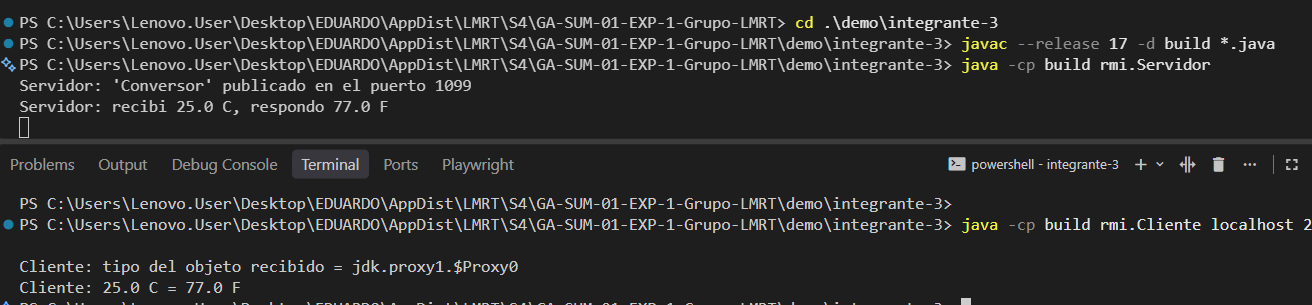
\includegraphics[width=.88\linewidth]{../evidencias/integrante-3/demo-rmi/01-demo-rmi.png}
\end{frame}

\begin{frame}{\proyectoTres · arquitectura propuesta (vista parcial)}\relax
{\footnotesize\textbf{Actualmente}\quad Plataforma web de selección de docentes no titulares de la UTEQ: 10 módulos, 52 controladores REST y 254 mapeos de endpoints (conteo propio, commit \texttt{86a238b}).}
\par\smallskip
\centering
\resizebox{.82\linewidth}{!}{% Diagrama propio de Eduardo Reinoso Vélez, derivado del bosquejo a mano del 20-11-2026.
% Vista parcial del SSDC: solo el flujo de verificación por correo. Lo punteado grueso es supuesto, no implementado.
\begin{tikzpicture}[
  x=1cm,y=1cm,
  bloque/.style={draw=Azul!60,fill=Bruma,rounded corners=2pt,
    align=center,text width=2.5cm,minimum height=1.05cm,inner sep=4pt,font=\fontsize{9}{10.5}\selectfont},
  flujo/.style={-{Stealth[length=2mm]},thick,draw=Azul},
  rotulo/.style={font=\fontsize{7.5}{9}\selectfont,align=center,text=Tinta}
]
\node[bloque] (front) at (0,0) {\textbf{Frontend Angular}\\\texttt{registro.ts}};
\node[bloque] (back) at (4.4,0) {\textbf{Backend}\\Spring Boot\\stub RMI};
\node[bloque,fill=white] (reg) at (9.5,.95) {\textbf{Registro RMI}\\puerto 1099};
\node[bloque,fill=white] (ver) at (9.5,-.95) {\textbf{Verificación remota}\\servidor RMI};
\node[bloque,fill=white] (smtp) at (4.4,-2.35) {\textbf{Servidor SMTP}\\Gmail};
\draw[draw=Azul!65,dashed,rounded corners=3pt] (-1.5,-.9) rectangle (1.5,.9);
\node[rotulo,anchor=south] at (0,.93) {Navegador};
\draw[draw=Azul!65,dashed,rounded corners=3pt] (2.7,-.9) rectangle (6.1,.9);
\node[rotulo,anchor=south] at (4.4,.93) {JVM del backend};
\draw[draw=Pendiente!80,dash pattern=on 4pt off 2pt,very thick,rounded corners=3pt] (7.85,-1.75) rectangle (11.15,1.85);
\node[rotulo,anchor=south,text=Pendiente] at (9.5,1.88) {\textbf{Supuesto, no implementado}\\JVM remota};
\draw[flujo] (front.east) -- node[above,rotulo]{HTTP POST} (back.west);
\draw[flujo] ([yshift=2mm]back.east) -- node[above=1pt,rotulo,sloped,pos=.5]{lookup} (reg.west);
\draw[flujo] ([yshift=-2mm]back.east) -- node[below=3pt,rotulo,sloped,pos=.6]{llamada al método} (ver.west);
\draw[flujo] (back.south) -- node[right,rotulo]{SMTP} (smtp.north);
\node[rotulo,anchor=north] at (9.5,-1.8) {Genera y valida códigos};
\end{tikzpicture}
}
\end{frame}

\begin{frame}{Decisiones al distribuir el SSDC (supuesto)}\relax
\small
\begin{tabularx}{\linewidth}{@{}lX@{}}
\toprule
Comunicación & RMI con llamada bloqueante; ambos extremos serían Java.\\
Transparencias & \textbf{Ofrecida:} acceso, la llamada parece local. \textbf{Limitada:} fallos; el usuario vería el error 500 de \texttt{VerificacionController} (líneas 28 a 31).\\
CAP & Una instancia y sin réplicas: no asigno etiqueta. Con réplicas y el enlace cortado: consistencia, se rechaza el código.\\
PACELC & Red sana: sin disyuntiva con una instancia, pero cada llamada suma latencia. No medida.\\
\bottomrule
\end{tabularx}
\end{frame}

\begin{frame}{Fallo hipotético y lección para el SSDC}\relax
\small
\textbf{Escenario}\quad El servicio remoto se reinicia entre generar y validar el código.\par\smallskip
\textbf{Causa raíz}\quad El código solo vive en memoria (\texttt{ConcurrentHashMap}, línea 17).\par\smallskip
\textbf{Respuesta}\quad \texttt{RemoteException}, reintento acotado, pedir código nuevo.\par\smallskip
\textbf{Comparación}\quad Redis guarda la clave con tiempo de vida y la borra al vencer \cite{redisexpire}. Compromiso: un servicio más que operar.\par\smallskip
\textbf{Lección}\quad Unir los dos mapas en uno con expiración, sin RMI. Prueba pendiente: esperar más de 10 minutos y validar.\par
\end{frame}
